\documentclass{article}

% Remember to also load the algostyle.sty file into your project.
\usepackage{algostyle}

% Insert new packages here.

\begin{document}
\begin{question}
Suppose that every student in your lab knows at least one other student. A student $X$ {\em distantly knows} student $Y$ if there exist a chain of students from $X$, who each directly know the next student in the chain, to $Y$. For example, if $X$ knows $Z$ and $Z$ knows $Y$, then $X$ distantly knows $Y$ even if they do not directly know each other. Two students $X$ and $Y$ {\em mutually} distantly know each other if $X$ distantly knows $Y$ and $Y$ distantly knows $X$.

Gerald claims that every student in the lab mutually distantly knows every other student and has come up with the following proof.
\begin{proof}[``Proof''.]
We prove that every student mutually distantly knows every other student via induction on the number of students. The base case is $n = 2$, which is true since every student knows at least one other student. Therefore, the two students must know each other which implies that they mutually distantly know each other.

Suppose that the claim is true for all subsets of $k$ students. Consider a group of $(k + 1)$ students. By the inductive step, the first $k$ students in the group mutually distantly know each other. Since the $(k + 1)$th student cannot know no one, they must know at least one person in the group who mutually distantly knows every other person in the group. Therefore, the $(k + 1)$th student also mutually distantly knows every other person, which completes the induction.
\end{proof}

However, there is a flaw in this proof. Can you find at least one counterexample? What went wrong in the proof?
\end{question}

\begin{solution}
    There is an important difference between the two phrases ``a group of students'' 
    and ``a group of students where each student knows at least one other''. The inductive hypothesis 
    only applies to the latter. 
    
    During the inductive step, the proof makes the claim that the first $k$ students must mutually distantly know each other. 
    However this is only true if upon removing the $(k + 1)$th student, the remaining $k$ students forms a 
    ``group of students where each student knows at least one other''. However, this is not the case if one
    of the first $k$ student \emph{only} knows the $(k+1)$th student.

    A counter example is the group of students represented by the diagram below, where an arrow from student $x$ to student $y$ indicates that $x$ knows $y$.

    

\begin{center}
    

\tikzset{every picture/.style={line width=0.75pt}} %set default line width to 0.75pt        

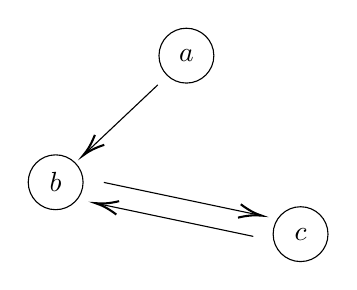
\begin{tikzpicture}[x=0.75pt,y=0.75pt,yscale=-1,xscale=1]
\draw   (167,71.21) .. controls (167,63.92) and (172.92,58) .. (180.21,58) .. controls (187.51,58) and (193.43,63.92) .. (193.43,71.21) .. controls (193.43,78.51) and (187.51,84.43) .. (180.21,84.43) .. controls (172.92,84.43) and (167,78.51) .. (167,71.21) -- cycle ;
\draw    (166.43,85.29) -- (131.88,117.91) ;
\draw [shift={(130.43,119.29)}, rotate = 316.64] [color={rgb, 255:red, 0; green, 0; blue, 0 }  ][line width=0.75]    (10.93,-3.29) .. controls (6.95,-1.4) and (3.31,-0.3) .. (0,0) .. controls (3.31,0.3) and (6.95,1.4) .. (10.93,3.29)   ;
\draw    (140.43,132.29) -- (214.47,147.87) ;
\draw [shift={(216.43,148.29)}, rotate = 191.89] [color={rgb, 255:red, 0; green, 0; blue, 0 }  ][line width=0.75]    (10.93,-3.29) .. controls (6.95,-1.4) and (3.31,-0.3) .. (0,0) .. controls (3.31,0.3) and (6.95,1.4) .. (10.93,3.29)   ;
\draw    (212.43,158.29) -- (138.39,142.7) ;
\draw [shift={(136.43,142.29)}, rotate = 11.89] [color={rgb, 255:red, 0; green, 0; blue, 0 }  ][line width=0.75]    (10.93,-3.29) .. controls (6.95,-1.4) and (3.31,-0.3) .. (0,0) .. controls (3.31,0.3) and (6.95,1.4) .. (10.93,3.29)   ;
\draw   (104,132.21) .. controls (104,124.92) and (109.92,119) .. (117.21,119) .. controls (124.51,119) and (130.43,124.92) .. (130.43,132.21) .. controls (130.43,139.51) and (124.51,145.43) .. (117.21,145.43) .. controls (109.92,145.43) and (104,139.51) .. (104,132.21) -- cycle ;
\draw   (222,157.21) .. controls (222,149.92) and (227.92,144) .. (235.21,144) .. controls (242.51,144) and (248.43,149.92) .. (248.43,157.21) .. controls (248.43,164.51) and (242.51,170.43) .. (235.21,170.43) .. controls (227.92,170.43) and (222,164.51) .. (222,157.21) -- cycle ;
\draw (180.21,71.21) node    {$a$};
\draw (117.21,132.21) node    {$b$};
\draw (235.21,157.21) node    {$c$};
\end{tikzpicture}
\end{center}
    
The proof would make the incorrect claim during the inductive hypothesis that upon the removal of $c$, the remaining 
set of students $\{a, b\}$ would form a group of students where all students know at least one other. 
Hence we see that $a$ and $c$ do not mutually know each other.

\end{solution}
\end{document}